\documentclass[border=10pt]{standalone}
\usepackage{tikz}
\usepackage{xcolor}
\usepackage{amsmath}

\begin{document}
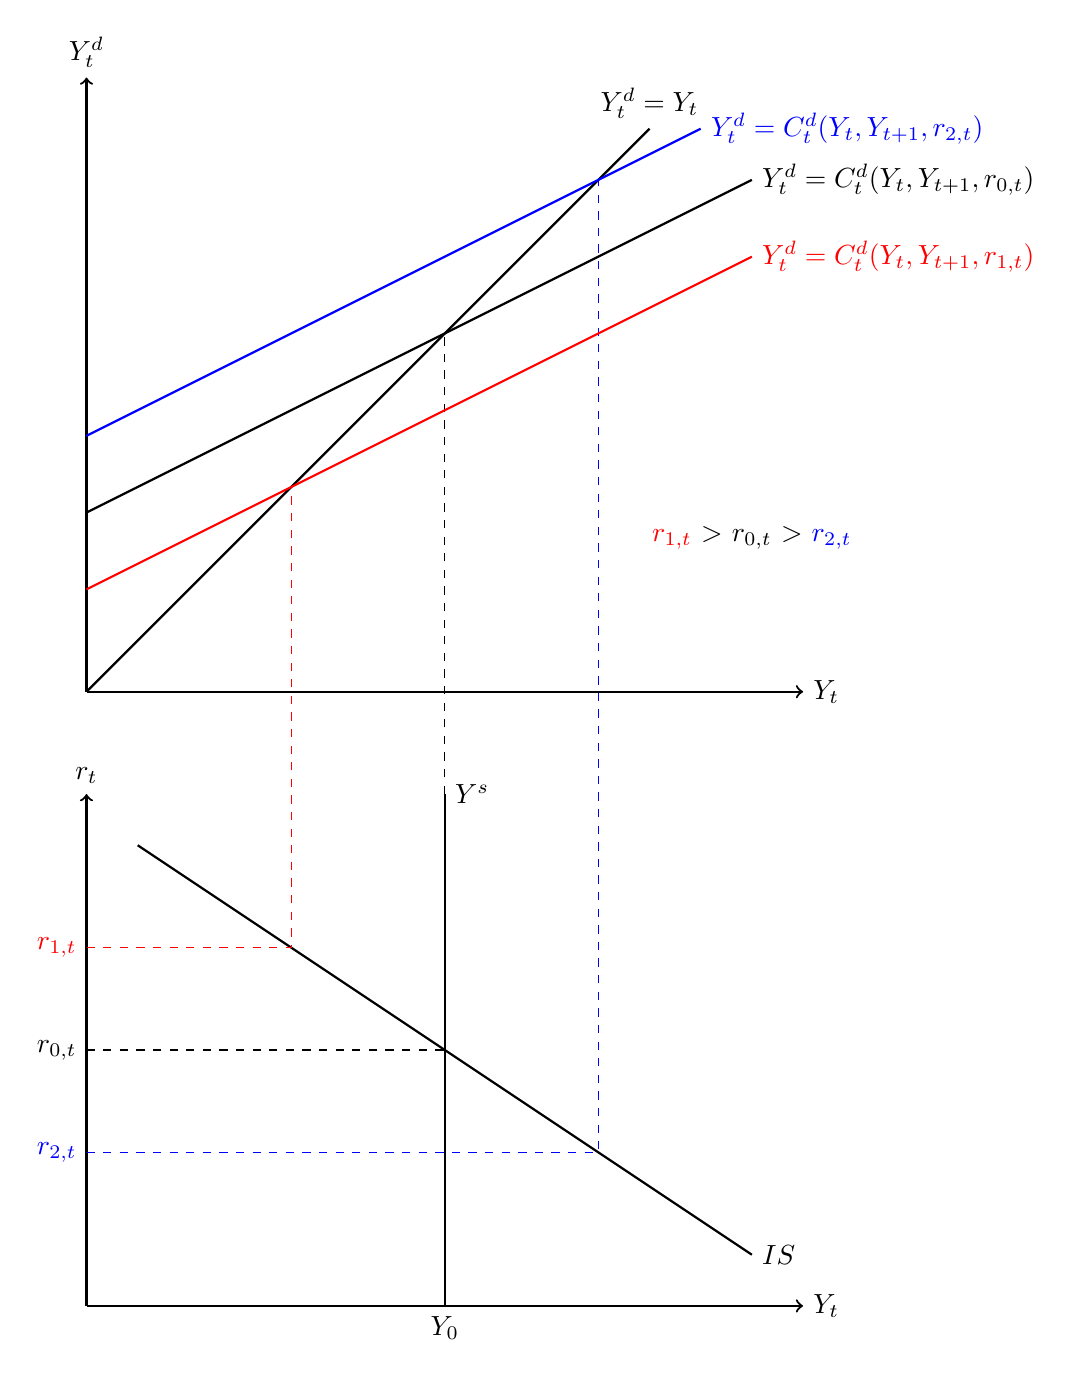
\begin{tikzpicture}[scale=1.3]

    % ==========================================
    % BOTTOM GRAPH: IS Curve Derivation
    % ==========================================
    
    % Axes
    \draw[thick, ->] (0,0) -- (7,0) node[right] {$Y_t$};
    \draw[thick, ->] (0,0) -- (0,5) node[above] {$r_t$};

    % IS Curve
    \draw[thick] (0.5, 4.5) -- (6.5, 0.5) node[right] {$IS$};

    % Y^s Vertical Line
    \draw[thick] (3.5, 0) node[below] {$Y_0$} -- (3.5, 5) node[right] {$Y^s$};

    % Dashed lines and interest rate labels
    % High interest rate (r1) -> low output
    \draw[dashed, red] (0, 3.5) node[left] {$r_{1,t}$} -- (2, 3.5) -- (2, 8);
    
    % Equilibrium interest rate (r0) -> medium output
    \draw[dashed, black] (0, 2.5) node[left] {$r_{0,t}$} -- (3.5, 2.5) -- (3.5, 9.5);
    
    % Low interest rate (r2) -> high output
    \draw[dashed, blue] (0, 1.5) node[left] {$r_{2,t}$} -- (5, 1.5) -- (5, 11);


    % ==========================================
    % TOP GRAPH: Keynesian Cross
    % ==========================================
    
    % Shift coordinate system up by 6cm for the top graph
    \begin{scope}[yshift=6cm]
        % Axes
        \draw[thick, ->] (0,0) -- (7,0) node[right] {$Y_t$};
        \draw[thick, ->] (0,0) -- (0,6) node[above] {$Y_t^d$};

        % 45-degree line (Y = Y^d)
        \draw[thick] (0,0) -- (5.5, 5.5) node[above] {$Y_t^d = Y_t$};

        % Aggregate Demand Curves
        % Bottom AD curve (Red - highest interest rate)
        \draw[thick, red] (0, 1) -- (6.5, 4.25) node[right] {$Y_t^d = C_t^d(Y_t, Y_{t+1}, r_{1,t})$};
        
        % Middle AD curve (Black - middle interest rate)
        \draw[thick, black] (0, 1.75) -- (6.5, 5.0) node[right] {$Y_t^d = C_t^d(Y_t, Y_{t+1}, r_{0,t})$};
        
        % Top AD curve (Blue - lowest interest rate)
        \draw[thick, blue] (0, 2.5) -- (6.0, 5.5) node[right] {$Y_t^d = C_t^d(Y_t, Y_{t+1}, r_{2,t})$};

        % Inequality text indicating the relationship between interest rates
        \node at (6.5, 1.5) {\textcolor{red}{$r_{1,t}$} $>$ $r_{0,t}$ $>$ \textcolor{blue}{$r_{2,t}$}};
    \end{scope}

\end{tikzpicture}
\end{document}